\section{Question 1}
\begin{enumerate}[label=(\alph*)]
    \item Write down the definition of \textbf{norm} for a vector space.
        \begin{solution}{}{}
            Let $\mX$ be a real vector space. A nonnegative-valued function $\norm{\cdot}: \mX\to\RR$ is called a norm if $\forall\vx,\vy\in\mX, \lambda\in\RR$
            \begin{itemize}
                \item $\norm{\lambda\vx}=\abs{\lambda}\norm{\vx}$ (absolutely homogeneous);
                \item $\norm{\vx+\vy}\leq\norm{\vx}+\norm{\vy}$ (triangle inequality);
                \item $\norm{\vx}=0\Rightarrow\vx =\va{0}$ (positive definite).
            \end{itemize}
            Moreover, the vector norm $\norm{\cdot}_p$ for $p=1,2,\ldots$ is defined as
            \[
                \norm{\vx}_p = \qty(\sum_{1\leq i\leq n}\abs{x_i}^p)^{1/p}.
            \]
            And the pair $(\mX, \norm{\cdot})$ is called a normed space.
        \end{solution}
    \item Given $\vx\in\RR^n$, show that followings are norm on $\RR^n$.
        \begin{enumerate}[label=\roman*.]
            \item $\norm{\vx}_\infty=\max_{1\leq i\leq n}\abs{x_i}$;
                \begin{solution}{}{}
                    \begin{itemize}
                        \item $\norm{\lambda\vx}_\infty=\max_{1\leq i\leq n}\abs{\lambda x_i}=\abs{\lambda}\max_{1\leq i\leq n}\abs{x_i}=\abs{\lambda}\norm{\vx}_\infty$
                        \item $\norm{\vx+\vy}_\infty=\max_{1\leq i\leq n}\abs{x_i+y_i}\leq\max_{1\leq i\leq n}\abs{x_i}+\max_{1\leq i\leq n}\abs{y_i}=\norm{\vx}_\infty+\norm{\vy}_\infty$
                        \item $\norm{\vx}_\infty=\max_{1\leq i\leq n}\abs{x_i}=0\Rightarrow\abs{x_i}=0\text{ where $1\leq i\leq n$}\Rightarrow\vx =\va{0}$
                    \end{itemize}
                \end{solution}
            \item $\norm{\vx}_1=\sum_{1\leq i\leq n}\abs{x_i}$;
                \begin{solution}{}{}
                    \begin{itemize}
                        \item $\norm{\lambda\vx}_1=\sum_{1\leq i\leq n}\abs{\lambda x_i}=\abs{\lambda}\sum_{1\leq i\leq n}\abs{x_i}=\abs{\lambda}\norm{\vx}_1$
                        \item $\norm{\vx+\vy}_1=\sum_{1\leq i\leq n}\abs{x_i+y_i}\leq\sum_{1\leq i\leq n}\abs{x_i}+\sum_{1\leq i\leq n}\abs{y_i}=\norm{\vx}_1+\norm{\vy}_1$
                        \item $\norm{\vx}_1=\sum_{1\leq i\leq n}\abs{x_i}=0\Rightarrow\abs{x_i}=0\text{ where $1\leq i\leq n$}\Rightarrow\vx =\va{0}$
                    \end{itemize}
                \end{solution}
            \item $\norm{\vx}_2=\qty(\sum_{1\leq i\leq n}\abs{x_i}^2)^{1/2}$.
                \begin{solution}{}{}
                    \begin{itemize}
                        \item $\norm{\lambda\vx}_2=\qty(\sum_{1\leq i\leq n}\abs{\lambda x_i}^2)^{1/2}=\abs{\lambda}\qty(\sum_{1\leq i\leq n}\abs{x_i}^2)^{1/2}=\abs{\lambda}\norm{\vx}_2$
                        \item $\norm{\vx+\vy}_2=\qty(\sum_{1\leq i\leq n}\abs{x_i+y_i}^2)^{1/2}\leq\qty(\sum_{1\leq i\leq n}\abs{x_i}^2)^{1/2}+\qty(\sum_{1\leq i\leq n}\abs{y_i}^2)^{1/2} = \norm{\vx}_2+\norm{\vy}_2$
                        \item $\norm{\vx}_2=\qty(\sum_{1\leq i\leq n}\abs{x_i}^2)^{1/2}=0\Rightarrow\sum_{1\leq i\leq n}\abs{x_i}^2\Rightarrow\vx =\va{0}$
                    \end{itemize}
                \end{solution}
        \end{enumerate}
        Plot the regions for $\norm{\vx}_p\leq 1$ in $\RR^2$ for $p=\infty,1,2$ respectively.
        \begin{figure}[H]
            \centering
            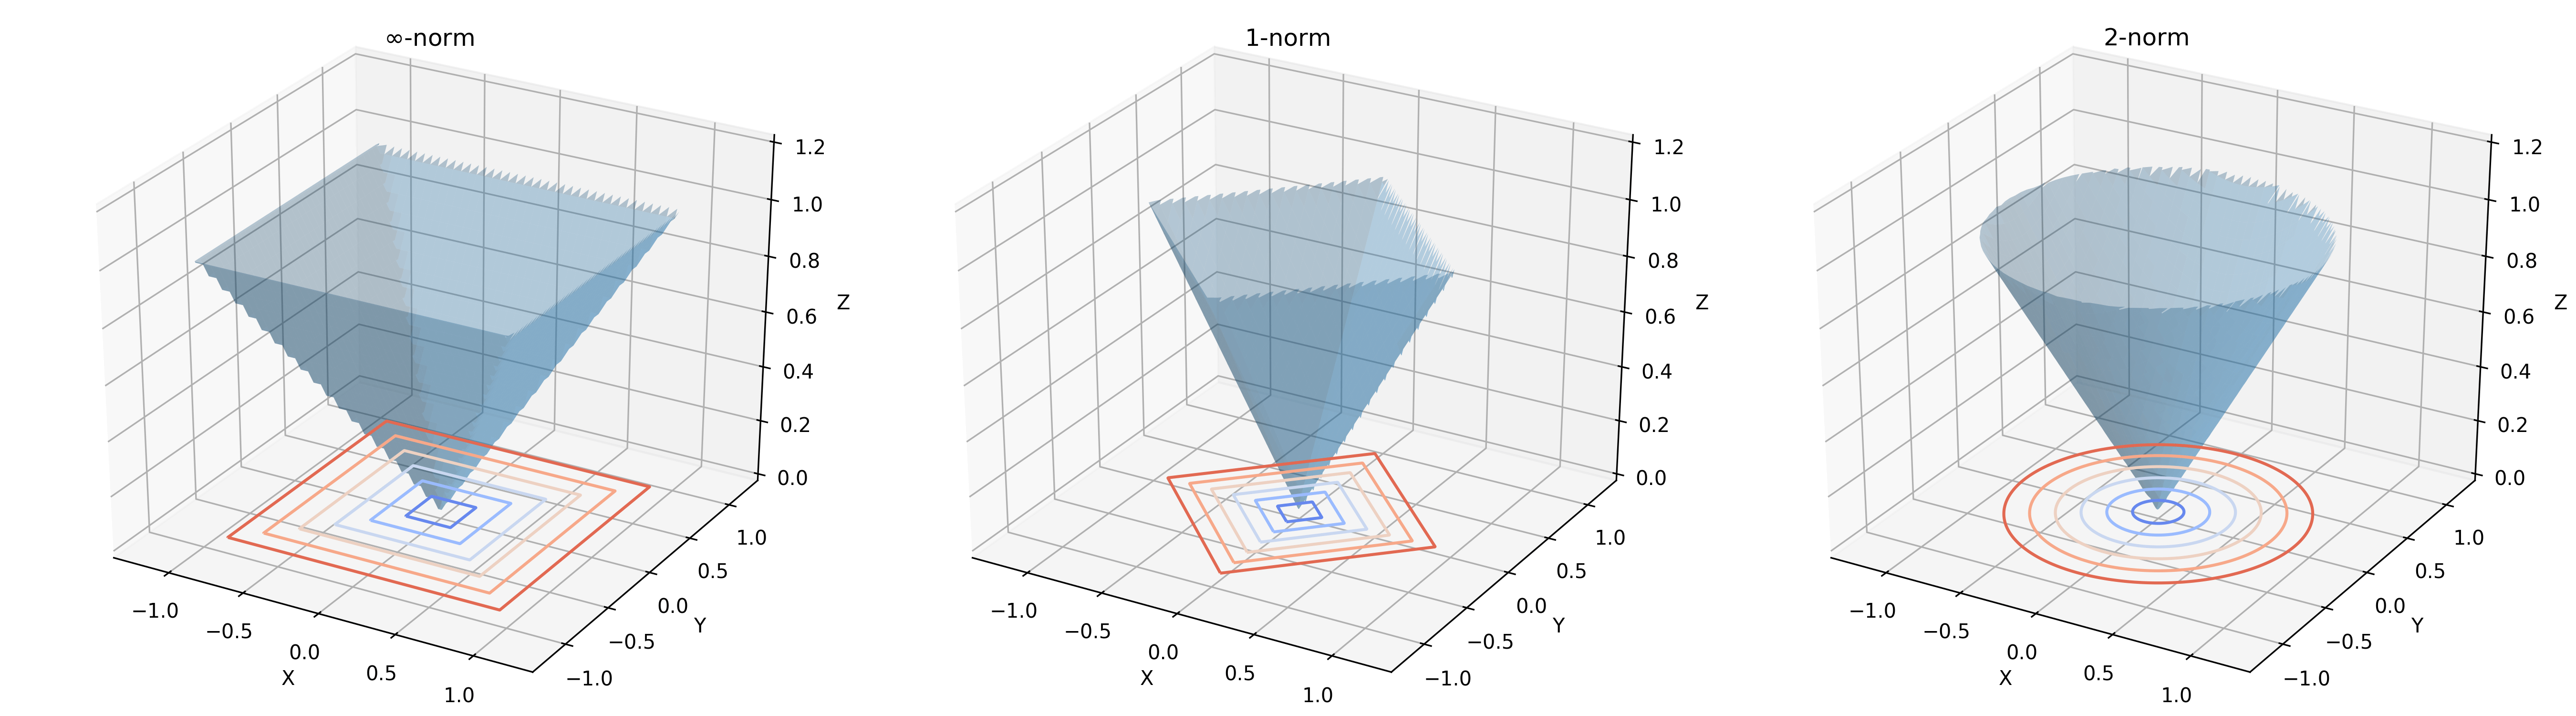
\includegraphics[width=.9\textwidth]{figures/1-1}
            \caption{Please refer to Appendix~\ref{S:appendix-1}}
        \end{figure}
    \item Given the vector norm $\norm{\cdot}_p$ for $\RR^n$, the induced norm for matrices $\mA\in\RR^{n\times n}$ is defined as
        \[
            \norm{\mA}_p = \max_{\vx\neq 0}\frac{\norm{\mA\vx}_p}{\norm{\vx}_p} = \max_{\norm{\vx}_p=1}\norm{\mA\vx}_p.
        \]
        Show that
        \begin{enumerate}[label=\roman*.]
            \item $\norm{\mA}_\infty=\max_{1\leq i\leq n}\sum_{j=1}^n\abs{a_{ij}}$;
                \begin{solution}{}{}
                    \begin{align*}
                        \norm{\mA}_\infty &= \max_{\norm{\vx}_\infty=1}\norm{\mA\vx}_\infty \\
                        &= \max_{\max_{1\leq j\leq n}\abs{x_j}=1}\max_{1\leq i\leq n}\sum_{j=1}^n\abs{a_{ij}x_j} \\
                        &\leq \max_{1\leq i\leq n}\sum_{j=1}^n\abs{a_{ij}} \\
                    \end{align*}
                    The equality holds when $x_j=\pm 1$ for $j=1,2,\ldots,n$.
                \end{solution}
            \item $\norm{\mA}_1=\max_{1\leq j\leq n}\sum_{i=1}^n\abs{a_{ij}}$;
                \begin{solution}{}{}
                    \begin{align*}
                        \norm{\mA}_1 &= \max_{\norm{\vx}_1=1}\norm{\mA\vx}_1 \\
                        &= \max_{\sum_{j=1}^n\abs{x_j}=1}\sum_{i=1}^n\sum_{j=1}^n\abs{a_{ij}x_j} \\
                        &\leq \max_{\sum_{j=1}^n\abs{x_j}=1}\sum_{j=1}^n\sum_{i=1}^n\abs{a_{ij}}\abs{x_j} = \max_{\sum_{j=1}^n\abs{x_j}=1}\sum_{j=1}^n\abs{x_j}\sum_{i=1}^n\abs{a_{ij}} \\
                        &\leq \max_{\sum_{j=1}^n\abs{x_j}=1}\sum_{j=1}^n\abs{x_j}\max_{1\leq j\leq n}\sum_{i=1}^n\abs{a_{ij}} = \max_{1\leq j\leq n}\sum_{i=1}^n\abs{a_{ij}}
                    \end{align*}
                    The equality holds when $j=\argmax_{1\leq j\leq n}\sum_{i=1}^n\abs{a_{ij}}$.
                \end{solution}
            \item $\norm{\mA}_2=\sqrt{\lambda_{\max}\qty(\mA^T\mA)}$.
                \begin{solution}{}{}
                    $\mA$ can be decomposed as $\vb{U}\vb*{\Sigma}\vb{V}^T$ by singular value decomposition, and the singular values on the diagonal are decreasing from top left to bottom right.
                    \begin{align*}
                        \norm{\mA}_2^2 &= \max_{\norm{\vx}_2=1} \norm{\mA\vx}_2^2 \\
                        &= \max_{\norm{\vx}_2=1} \qty(\mA\vx)^T\mA\vx = \max_{\norm{\vx}_2=1}\vx^T\vb{V}\vb*{\Sigma}^2\vb{V}^T\vx \\
                        &= \max_{\norm{\vx}_2=1}\vy^T\vb*{\Sigma}\vy = \max_{\norm{\vx}_2=1}\sum_{i=1}^n\sigma_iy_i^2 \\
                        &\leq \max_{\norm{\vx}_2=1}\max_{1\leq i\leq n}\sigma_i \vy^T\vy = \max_{\norm{\vx}_2=1}\max_{1\leq i\leq n}\sigma_i \vx^T\vx\\
                        &= \max_{1\leq i\leq n}\sigma_i = \lambda_{\max}\qty(\mA^T\mA).
                    \end{align*}
                    The equality holds when $\vx=\vb{V}\vb{e}_1$, where $\vb{e}_1=[1,0,\ldots,0]^T$.
                \end{solution}
        \end{enumerate}
\end{enumerate}



\section{Question 2}
\begin{enumerate}[label=(\alph*)]
    \item Use the method of undetermined coefficients to design third order accurate approximation to $u'(\bar{x})$ by using the discrete points $\bar{x}+h$, $\bar{x}$, $\bar{x}-h$, $\bar{x}-2h$.
        \begin{solution}{}{}
            According to Appendix~\ref{S:appendix-1}, we have
            \[
                u'(\bar{x}) = \frac{1}{h}\qty(\frac{u(\bar{x}-2h)}{6}-u(\bar{x}-h)+\frac{u(\bar{x})}{2}+\frac{u(\bar{x}+h)}{3}).
            \]
        \end{solution}
    \item Assuming $u(x)$ is smooth enough, compute the truncation error (leading term) for the finite difference formula above.
        \begin{solution}{}{}
            The leading term of the truncation error is of $\order{h^3}$, that is
            \[
                \frac{h^3}{12}u^{(4)}(\bar{x}).
            \]
        \end{solution}
    \item What is the truncation error if $u(x) = 4x^4 + 12x^3 + 6x^2 + x/2 + \pi$.
        \begin{solution}{}{}
            \begin{align*}
                u'(\bar{x}) &= \frac{1}{h}\qty(\frac{u(\bar{x}-2h)}{6}-u(\bar{x}-h)+\frac{u(\bar{x})}{2}+\frac{u(\bar{x}+h)}{3}) \\
                &= 16\bar{x}^3 + 36\bar{x}^2 + 12\bar{x} + \frac{1}{2}
            \end{align*}
            We have $u'(x)=16x^3 + 36x^2 + 12x + 1/2$, that is, the truncation error of this given function is $0$.
        \end{solution}
\end{enumerate}



\section{Question 3}
\begin{enumerate}[label=(\alph*)]
    \item For the following $N\times N$ matrix, show that all eigenvalues are given by $\lambda_p = a+2b\cos\tfrac{\pi p}{N+1}$ for $p=1,2,\ldots,N$.
        \[
            \qty[\begin{NiceArray}{CCCC}
                a & b      &        &   \\
                b & \Ddots & \Ddots &   \\
                  & \Ddots & \Ddots & b \\
                  &        & b      & a \\
            \end{NiceArray}]_{N\times N}
        \]
        \begin{solution}{}{}
            Please refer to Section~\ref{Q:4-1}.
        \end{solution}
\end{enumerate}



\section{Question 4}\label{Q:4-1}
\begin{enumerate}[label=(\alph*)]
    \item For the following $N\times N$ matrix, show that all eigenvalues are given by $\lambda_p = a+2\sqrt{bc}\cos\tfrac{\pi p}{N+1}$ for $p=1,2,\ldots,N$ and $bc>1$.
        \[
            \qty[\begin{NiceArray}{CCCC}
                a & c      &        &   \\
                b & \Ddots & \Ddots &   \\
                  & \Ddots & \Ddots & c \\
                  &        & b      & a \\
            \end{NiceArray}]_{N\times N}
        \]
\end{enumerate}



\section{Question 5}
For the 2-point BVP with Neumann boundary conditions:
\[
    \begin{cases}
        u''(x) = f(x), & x\in(0, 1) \\
        u'(0) = u'(1) = 0 & \\
    \end{cases}
\]
\begin{enumerate}[label=(\alph*)]
    \item Set the grid points as $x_j=jh$ for $j=0,1,\ldots,N$ and $h=1/N$. Write down the central FD scheme for the main equation with using $u_j$ to approximate $u(x_j)$.
    \item\label{tmp-1} Add two ``ghost'' points as $x_{-1}=-h$ and $x_{N+1}=1+h$, and two more variables $u_{-1}$ and $u_{N+1}$. Treat the boundary condition as $(u_1-u_{-1})/2h=0$, $(u_{N+1}-u_{N-1})/2h=0$. Assemble all the equations as $\mA\vb{U}=\vb{F}$ where $\vb{U}=[u_0, u_1, \ldots, u_N]^T$.
    \item Show that $\mA$ is singular, and find out when the system $\mA\vb{U}=\vb{F}$ has solutions.
    \item Find the kernel space of $\mA$.
    \item Find out all eigenvalues and eigenvectors for the matrix $\mA$ given in \ref{tmp-1}.
\end{enumerate}



\section{Appendix}\label{S:appendix-1}
\begin{appendices}
    \pythonfile{code/hw1.py}{\texttt{hw1.py}}
    \pythonfile{code/1_2_sympy.py}{\texttt{1\_2\_sympy.py}}
\end{appendices}
